\newcommand{\TeamNo}{31}

\newcommand{\HWno}{02}

\newcommand{\AuthorOneName}{Merve Nur Öztürk}
\newcommand{\AuthorOneID}{2311322}

\newcommand{\AuthorTwoName}{Atakan Süslü}
\newcommand{\AuthorTwoID}{2311371}

\newcommand{\AuthorThreeName}{Betül Rana Kuran}
\newcommand{\AuthorThreeID}{2311173}


\documentclass[letterpaper,12pt]{article}
\usepackage{tabularx} % extra features for tabular environment
\usepackage{amsmath}  % improve math presentation
\usepackage{amssymb}
\usepackage{xcolor}
\usepackage{float}
\usepackage[export]{adjustbox}
\usepackage{graphicx} % takes care of graphic including machinery
\usepackage[margin=1in,letterpaper]{geometry} % decreases margins
\usepackage{cite} % takes care of citations

\begin{document}
\begin{center}
AE 305, 2020-21 Fall \hfill \textbf{HW \HWno} \hfill \textbf{Team \TeamNo} \\
\noindent\rule{\textwidth}{0.4pt}
\begin{tabular}{p{0.33\textwidth} | p{0.33\textwidth} | p{0.33\textwidth} }
	\AuthorOneName&\AuthorTwoName&\AuthorThreeName\\
	\textit{\AuthorOneID}&\textit{\AuthorTwoID}&\textit{\AuthorThreeID}
\end{tabular}
\noindent\rule{\textwidth}{0.4pt}
\end{center}

%Report start

\section{Introduction}


\section{Method}

\newpage

\section{Results and Discussion}

% Görmek için koydum, yazarken silin
\begin{figure}
	\centering
	\includegraphics[height = 8.5cm]{graphs/q1_pc.eps}
\end{figure}
\begin{figure}
	\centering
	\includegraphics[height = 8.5cm]{graphs/q1_isp.eps}
\end{figure}
\begin{figure}
	\centering
	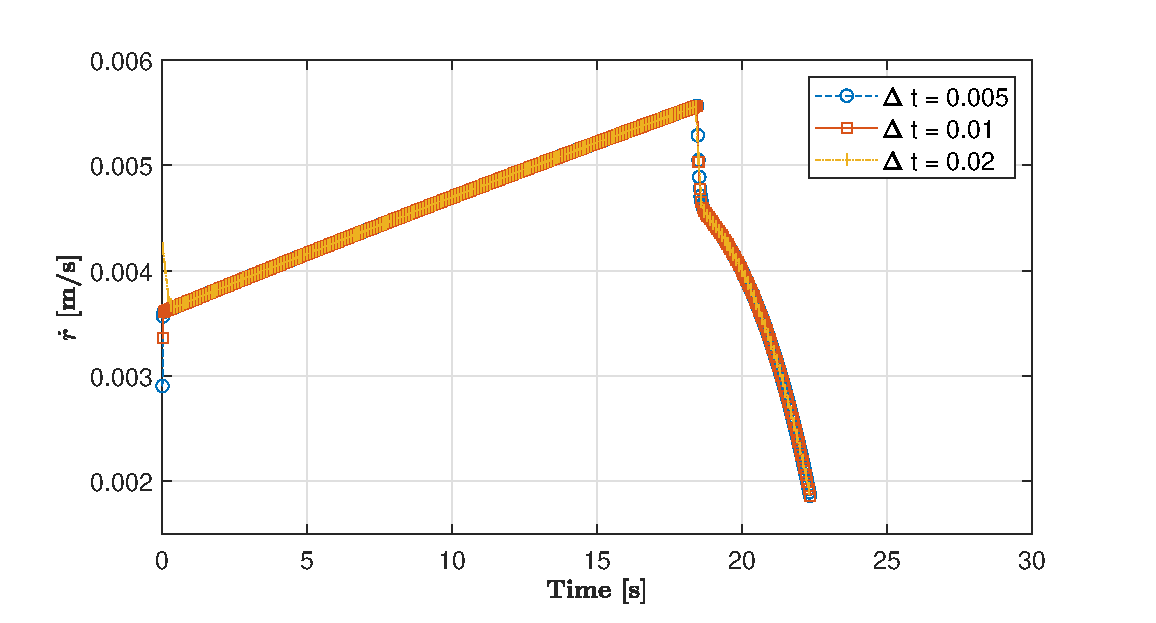
\includegraphics[height = 8.5cm]{graphs/q1_rdot.eps}
\end{figure}
\begin{figure}
	\centering
	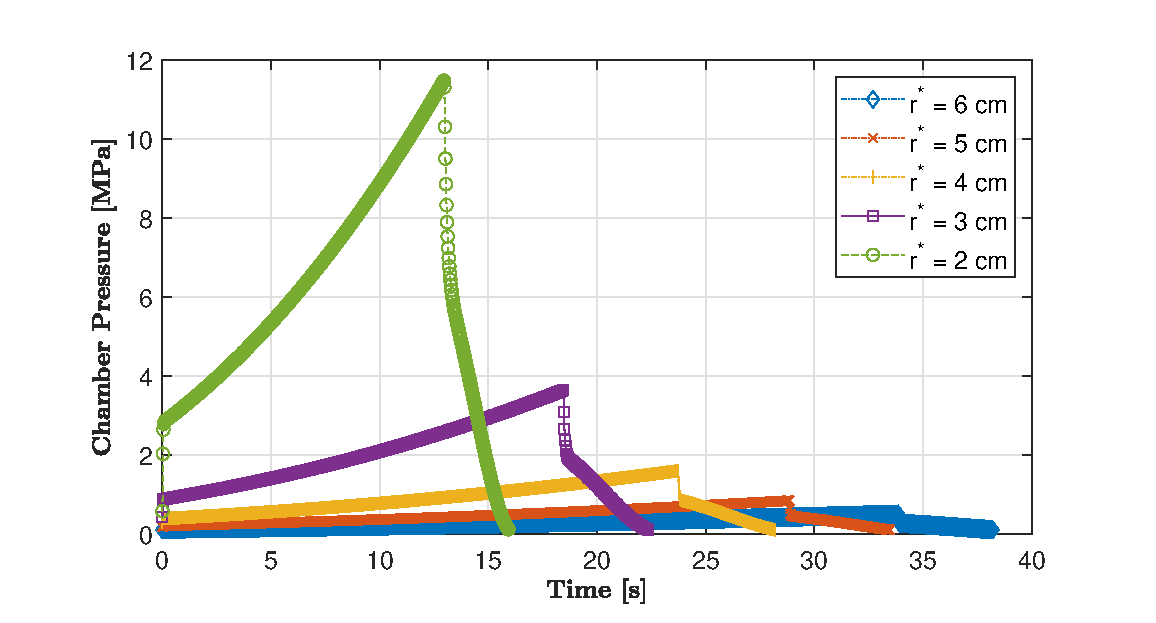
\includegraphics[height = 8.5cm]{graphs/q2_pc.eps}
\end{figure}
\begin{figure}
	\centering
	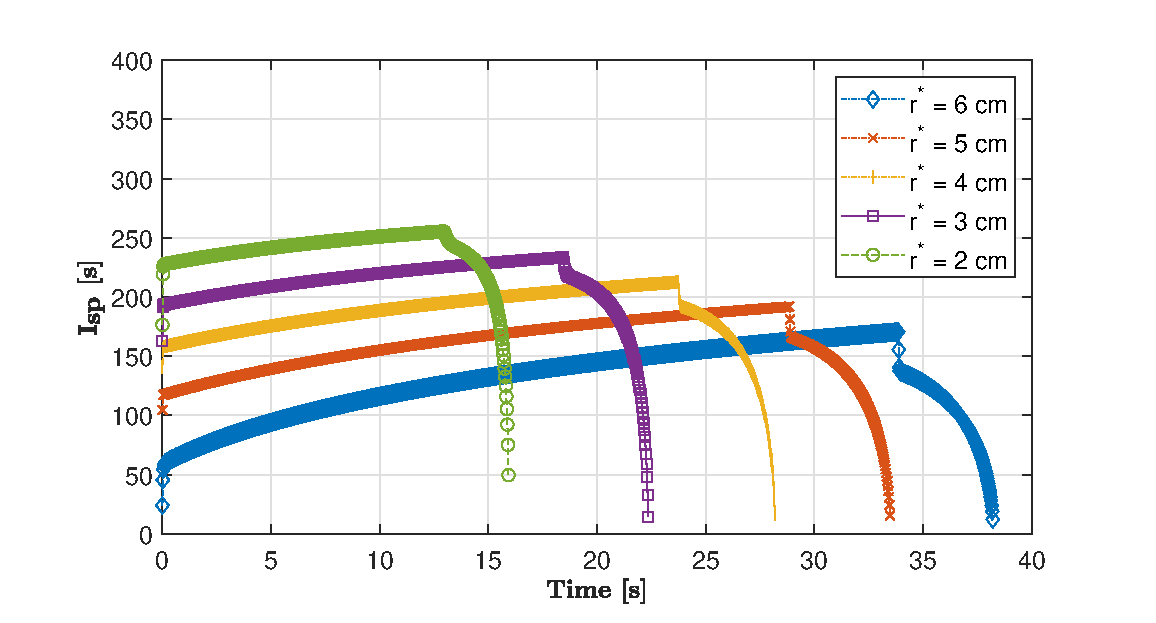
\includegraphics[height = 8.5cm]{graphs/q2_isp.eps}
\end{figure}
\begin{figure}
	\centering
	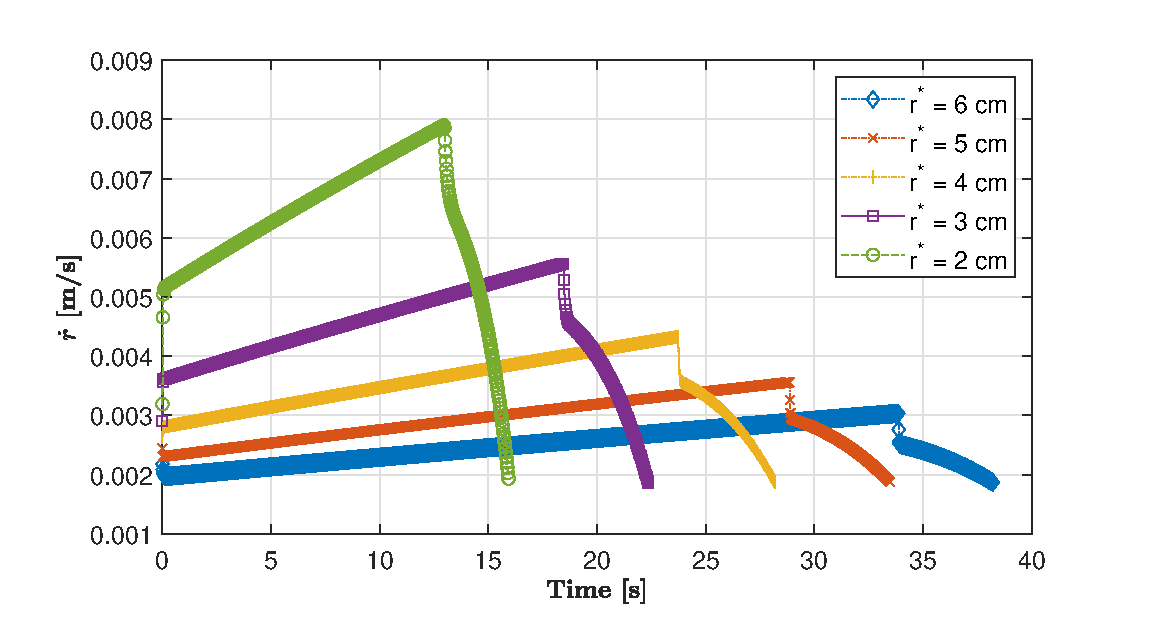
\includegraphics[height = 8.5cm]{graphs/q2_rdot.eps}
\end{figure}
\section{Conclusion}

\end{document}